% CVPR 2023 Paper Template
% based on the CVPR template provided by Ming-Ming Cheng (https://github.com/MCG-NKU/CVPR_Template)
% modified and extended by Stefan Roth (stefan.roth@NOSPAMtu-darmstadt.de)

\documentclass[10pt,twocolumn,letterpaper]{article}

%%%%%%%%% PAPER TYPE  - PLEASE UPDATE FOR FINAL VERSION
\usepackage[review]{cvpr}      % To produce the REVIEW version
%\usepackage{cvpr}              % To produce the CAMERA-READY version
%\usepackage[pagenumbers]{cvpr} % To force page numbers, e.g. for an arXiv version

% Include other packages here, before hyperref.
\usepackage{graphicx}
\usepackage{amsmath}
\usepackage{amssymb}
\usepackage{booktabs}


% It is strongly recommended to use hyperref, especially for the review version.
% hyperref with option pagebackref eases the reviewers' job.
% Please disable hyperref *only* if you encounter grave issues, e.g. with the
% file validation for the camera-ready version.
%
% If you comment hyperref and then uncomment it, you should delete
% ReviewTempalte.aux before re-running LaTeX.
% (Or just hit 'q' on the first LaTeX run, let it finish, and you
%  should be clear).
\usepackage[pagebackref,breaklinks,colorlinks]{hyperref}


% Support for easy cross-referencing
\usepackage[capitalize]{cleveref}
\crefname{section}{Sec.}{Secs.}
\Crefname{section}{Section}{Sections}
\Crefname{table}{Table}{Tables}
\crefname{table}{Tab.}{Tabs.}


%%%%%%%%% PAPER ID  - PLEASE UPDATE
\def\cvprPaperID{7421} % *** Enter the CVPR Paper ID here
\def\confName{CVPR}
\def\confYear{2023}


\begin{document}

%%%%%%%%% TITLE - PLEASE UPDATE
\title{Learning Knowledge Integration for Hierarchically Represented Diffusion \\ MRI Segmentation}

\author{First Author\\
Institution1\\
Institution1 address\\
{\tt\small firstauthor@i1.org}
% For a paper whose authors are all at the same institution,
% omit the following lines up until the closing ``}''.
% Additional authors and addresses can be added with ``\and'',
% just like the second author.
% To save space, use either the email address or home page, not both
\and
Second Author\\
Institution2\\
First line of institution2 address\\
{\tt\small secondauthor@i2.org}
}
\maketitle

%%%%%%%%% ABSTRACT
\begin{abstract}
Medical image processing has greatly influenced the efficiency of medical image analysis and diagnose. 
However, it is still facing the problem of insufficiency of training samples and noisy labeling. 
In order to obtain high quality and high resolution labels, we proposed a knowledge integration method to learn mask prediction and hierarchically edge representation from coarse labeled data. 

In this work, we take the task of diffusion MRI brain mask estimation. 
The problem is set as learning mask prediction from source dataset with coarse and noisy labels. 
% , and a supplementary dataset from another domain with standard labeling. 
we proposed a new method, including a new efficient network, 
% without skip connection which is wildly used in UNet and its variation, 
a new learning schedule for knowledge integration. 
Thus the learning system can learn knowledge from uncertain labels.

The results show significant improvements in both quantization and visualization, and the hierarchically edge representation shows great potential in human customized image segmentation.

\end{abstract}

%%%%%%%%% BODY TEXT
\section{Introduction}
\label{sec:intro}

During recent years medical image processing and recognition have prodigious progress with the advanced of deep learning and machine learning theory. 
Deep artificial neural networks have great improvements on the accuracy of natural image recognition and analysis. These improvements mainly benefit from the increasing huge amount of data and high performance computing. 
Medical image processing and recognition is a large research topic. 
Nevertheless, most of medical image related tasks are facing the same problem, lack of data and high quality annotation. 
Even though plenty of few-shot or zero-shot learning methods are proposed, but most of them are not robust enough, thus can not be easily applied to clinical usage. 


For medical image segmentation tasks, since high quality annotation is time-consuming and the difficulty for human to distinguish each pixel, the annotations are usually indistinct. 
In general view, the problem can be assigned as noisy labeling problem. 
But in fact, the ~\textbf{key knowledge are missing} in the labeling. 
In order to correct the unclear labels, additional knowledge should be integrated into the system. 

\begin{figure}[t]
  \centering
%   \fbox{\rule{0pt}{2in} \rule{0.9\linewidth}{0pt}}
   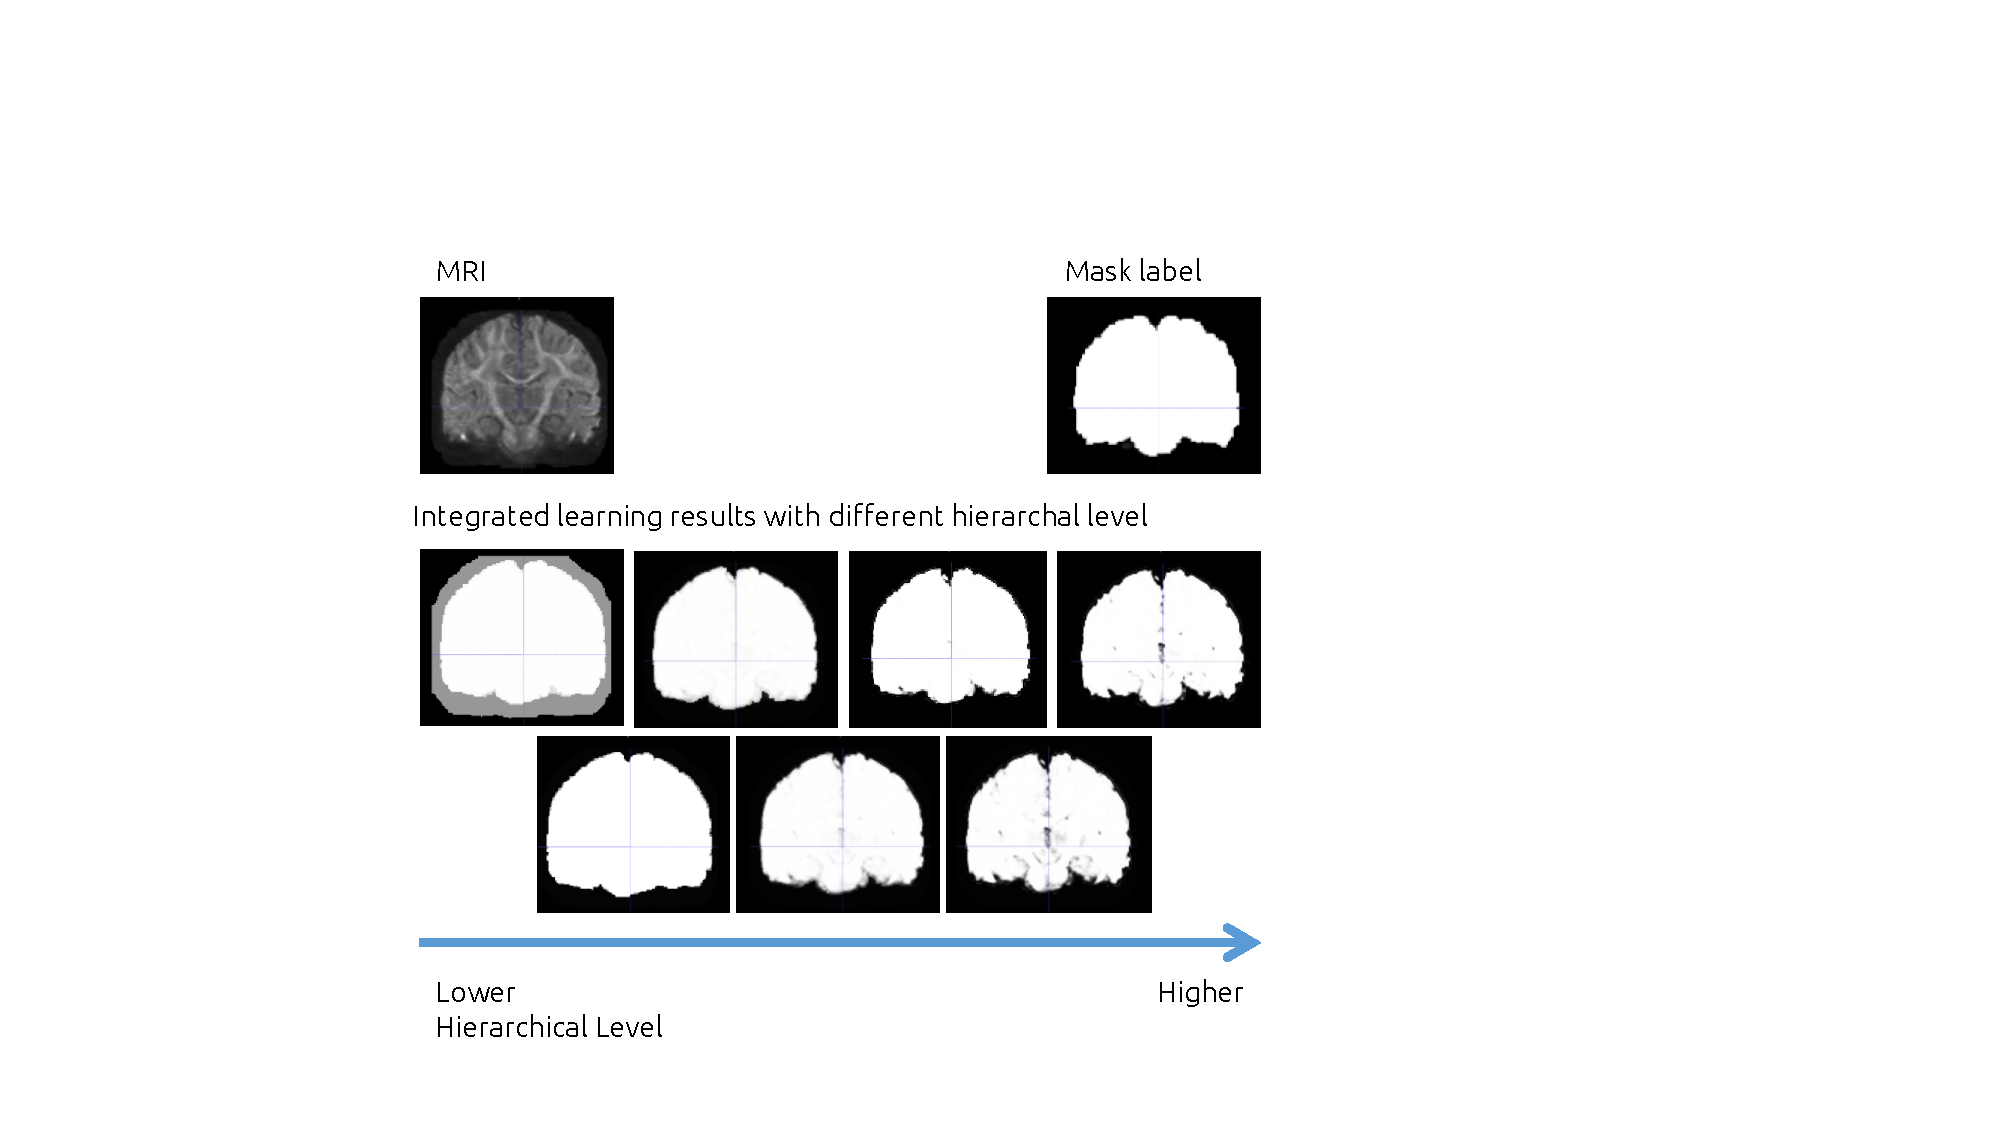
\includegraphics[width=1\linewidth]{./figs/first.pdf}
   \caption{\textbf{The visualization of knowledge integration learning based hierarchically representation results.} 
   Top left: MRI data. Top right: the coarse mask label of the MRI data. Bottom, from left to right: the result of hierarchically representation learning with different hierarchically levels. }
   \label{fig:first}
\end{figure}


To vividly understand it, we utilize a simple brain mask segmentation task. 
In detail, The dataset~\textit{A} is a brain MRI (diffusion MRI) dataset with indistinct masks, and the task is to estimate high quality masks according to the coarse masks.
% which is better than the ground truth. 
%, and the dataset~\textit{B} is a brain MRI dataset too but it is in another domain (T1 weighted). The dataset~\textit{B} has less samples but all the samples are well annotated by human. The purpose of the task is to predict the label of dataset~\textit{A} with utilizing the knowledge of dataset~\textit{B}. 
The problem can be resigned as ~\textbf{under-labeling} problem. 
In this work, new method to obtain the lacked knowledge is proposed for this problem. 
Since the edge of the diffusion MRI is blurry and uncertain, a new unsupervised hierarchical knowledge representation method is proposed to describe the abundant low-level texture information. Thus the deep model can learn abundant low-level image representation without extra manual annotations. 
As shown in Fig.~\cref{fig:first}, even though the mask annotation of the MRI is bluer and noisy, the learnt result masks can clearly represent the edge of the source image. 
This is mainly benefit from the hierarchically represented low-level knowledge and the proposed knowledge integration learning method. 
% Another benefit is that 
Further more, the hierarchical level can be further adjusted and selected during usage according to different applications. 
%a new method to integrate the source knowledge and the complementary knowledge is proposed. And the deep neural network can learn the integrate knowledge for exponential performance. 




\section{Related Background}

In this section, we provide brief introductions of related topics and background knowledge. 

\subsection{Medical Image Segmentation}
Medical image segmentation is an application of image segmentation. 
But it is differ from common nature image segmentation task. 
The most is the imaging style and the high dimension. Thus the general image segmentation model for nature image can not directly applied to medical image. 
And another issue is the gray level in medical image, which always refer to real physical property. 
Since the diagnose and analysis are actually based on the physicochemical property, the gray value itself is valuable. 
In order to obtain high quality voxel-wised analysis results, high quality and high resolution labeling is necessary for medical image. 

The labeling work for medical image require professional knowledge and huge workload compared with natural images. The cost is extremely high which greatly hinder the procedure. 
However, most works for both natural images and medical images are based on fully supervised methods which rely on huge amount labeling to achieve acceptable results. 
But the labels are uncertain even for an expert in many medicine tasks. As a result, a general deep learning model has to face huge amount noisy labels which greatly influence the reliability and robustness. 

In this work, a new method which utilize coarse labels to obtain high quality and high resolution image segmentation is proposed. Thus it can greatly reduce the cost of labeling work, while only slightly modification is necessary. 


\subsection{Deep Learning for Image Segmentation}

Deep learning methods obtains huge improvements for both semantic~\cite{Noh_2015_ICCV} and semantic independent segmentation~\cite{he2017mask, hong2015decoupled}. 
Huge amount of deep neural networks are proposed for this task in recent years. 
Most of them utilize encoder-decoder structure. 
In order to capture low-level texture information for high-resolution segmentation, skip connects~\cite{unet} and dilated convolution are proposed. 
However, both of them meet their disadvantages even though huge amount networks are proposed to alleviate this problem. 

In this work, a new combination of a spatial-squeeze network and a wide-squeeze network are proposed for capture global and texture information. 
Skip connection between encoder and decoder, and dilated convolution are avoid in case of under-fitting and grid effect. 

\subsection{Unsupervised Learning}
Unsupervised learning are wildly used for pre-train and transfer learning. A good initialization would greatly improve the performance of a deep neural network. 
However, currently most of the unsupervised learning and transfer learning dose not learn the knowledge directly related to the target tasks, and are served as a pre-train schedule. 

In this work, the label of the dataset are coarse and noisy, and the proposed unsupervised low-level representation learning can greatly improve the performance of image segmentation in edge areas. 


\subsection{Noisy Labeling}
Noisy labeling problem is a normal phenomenon in machine learning system. 
Noisy labels, including wrong labels, labels with large error or low quality labels can greatly decrease the performance of the whole system. 
Many methods are proposed to alleviate the influence of the noisy labels instead of removing them, since the data size is another factor related to the performance of the deep learning model. 
In the realistic application, for a new task, there are huge amount unlabeled or coarse labeled data, and there may be a small set of labeled data. A deep learning system is trained on all of the datasets in order to fit on various of source images. 
However, the performance of the deep neural networks trained on noisy data are always lower than which trained on clear data. 



\subsection{Knowledge Representation and Learning}

Knowledge representation and learning is a never-end topic in machine learning system. It is related to the design of the model, the loss function and also the labeling methods. 
For example, the one-hot labels for image classification, the high-dimension representation and distance measurement of metric-learning based deep learning models, and the bounding-box represented labels for object detection~\cite{Girshick_2015_ICCV}. 

Knowledge distillation is another example, in which one model can learn from others. 
In detail, a new network can obtain gradient from a well-trained network. Usually the new network is smaller and faster and the trained network is large. In the training procedure, the knowledge of the large network (also called "teacher" network) is distilled to the smaller network (called "student" network). 
In this procedure, the knowledge is transferred from one to another though the loss function between the output of the teacher and student network. 

\begin{figure*}[t]
  \centering
%   \fbox{\rule{0pt}{2in} \rule{0.9\linewidth}{0pt}}
   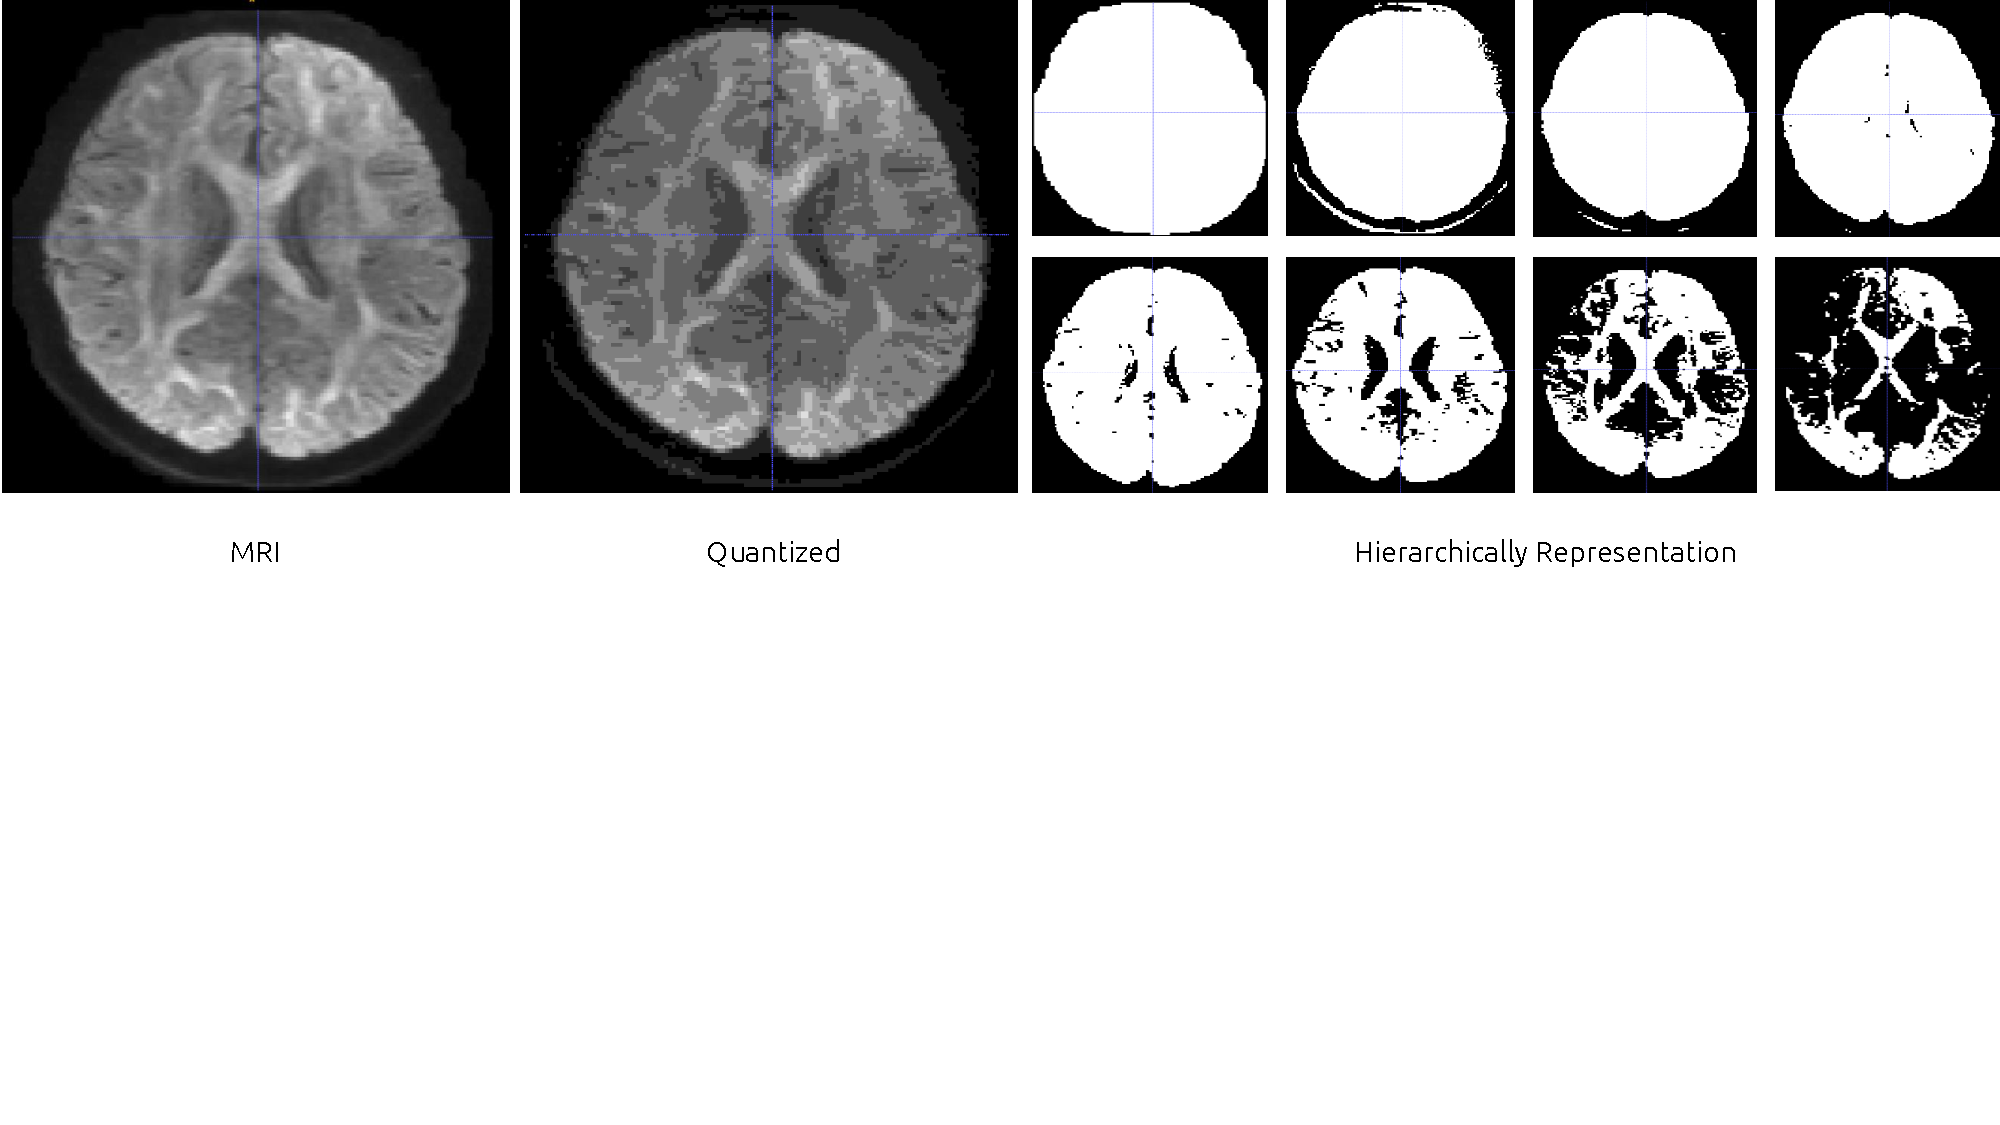
\includegraphics[width=1\linewidth]{./figs/HR.pdf}
   \caption{\textbf{The visualization of hierarchically representation maps.} 
   From left to right: the MRI, the quantized MRI and the hierarchically represented maps. }
   \label{fig:hr}
\end{figure*}


In another word, the output of the "teacher" network are served as dark-knowledge labels for training the student network. 
In this work, the knowledge is represented and learnt via a new learning schedule. The original coarse label knowledge and the hierarchically edge representation knowledge are integrated to produce better results. 

\section{Methods}

\subsection{Overview}

Denote the input as $X$, 


\subsection{Hierarchical Representation for Medical Image Segmentation}

 
MRI is a type of medical data with abundant details. These details are important for processing and diagnose. 
However, this information may not be learnt by the deep neural network directly. 
Even though some techniques such as skip-connection are proposed to force the deep neural network to focus on the low-level patterns. 

In this section, a new hierarchical representation method is proposed to help the neural networks to learn abundant low-level information. 
As shown in~\cref{fig:hr}, firstly the quantization of the MRI is calculated via transfer it into a $N$ bit image with $2^N$ gray levels. 
Here we show an 3 bit example with 8 gray levels. 
Then it can be sliced into the hierarchical representation, which is a set of images consist of 8 images. Each image represents one hierarchical level. 

Generalized speaking, those hierarchical representations show the contour lines of the image. Abundant edge information is encoded inside these contours. 
During training, these masks are used as unsupervised supervision. 
As a results, the edge knowledge can be encoded into the deep neural networks. 



\subsubsection{Knowledge Representation and Integration}








\subsubsection{The Spacial-Wide squeeze Network}


\begin{figure*}
  \centering
%   \begin{subfigure}{0.68\linewidth}
     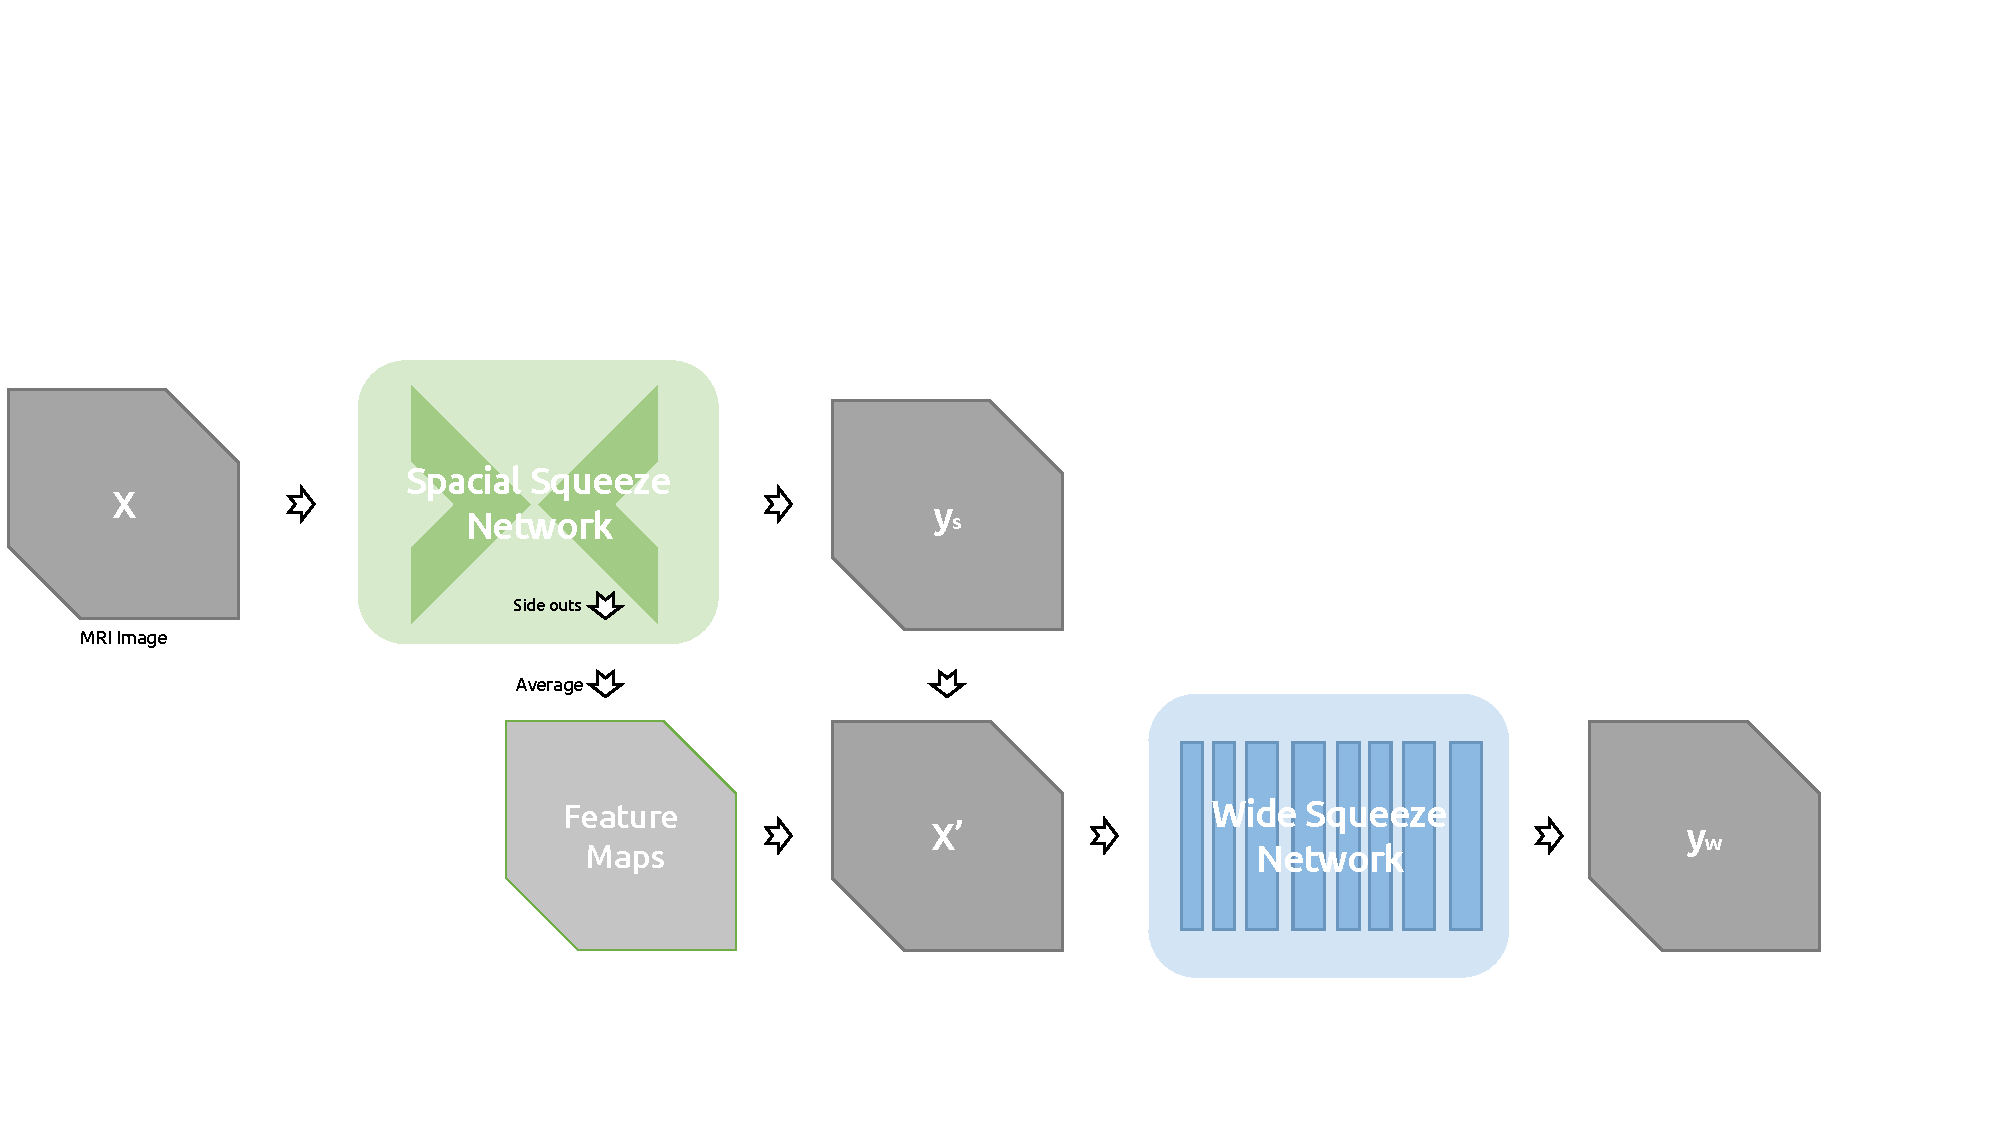
\includegraphics[width=1\linewidth]{./figs/main.pdf}
    \caption{\textbf{The illustration of the deep neural networks. } It includes a spacial-squeeze network and a wide-squeeze network. The spacial-squeeze network has a encoder-decoder architecture, and multi-level feature maps from the decoder are averaged across each block and then feed into the wide squeeze network together with the MRI image $X$ (not shown in the figure) and the output $y_s$. The wide-squeeze network keeps the spatial dimension and various across the channel dimension. }
    \label{fig:main}
\end{figure*}

As shown in Fig.~\cref{fig:main}, a new due path deep neural network is proposed. 
It includes a spacial-squeeze network (SCN) and a wide-squeeze network (WCN). 
The spacial-squeeze network utilize an encode-decoder structure, it obtains a larger receptive field for global information perception and is efficient. 
The wide-squeeze network squeeze and expand the feature maps across the channel dimension while the spacial dimensions are kept the same going through the layer. 
It take the original image $x$, the output of SCN $y$ and the averaged side-out feature maps as input. 
The output of the WCN is noted as $y_w$. 

In the SCN, a convolution layer with kernel size 2 and stride 2 are utilized as down sampling layer. 
The up-sample layer is a convolution layer follow with a reshape layer. 
Thus each pixel/ voxel in the up-sampled feature maps are calculated via the convolution layer. 
Pooling layer and interpolation operation are discarded here for better spacial perception ability. 
Furthermore, skip connections across the encoder and decoder which are commonly utilized in Unet and its variations are discard too. 
The reason is that the skip connection would decrease the equivalent depth of the deep neural networks. 

The output of SCN and its side-outs are served as the input of the WCN. 
The side-outs are from the last three layers of the decoder, and they are averaged into three single maps. 
The averaged side-outs, the output $y_s$ and the original image $X$ are concatenated as the input of WCN.
As shown in Fig.~\cref{fig:net2}, the channel dimension of the feature maps are squeezeed and expanded via convolution layers, and a extra convolution layer with the kernel size 3 is utilized in the wide squeeze layer. 








% {The illustration of the deep neural networks. } It includes a spacial-squeeze network and a wide-squeeze network. The spacial-squeeze network has a encoder-decoder architecture, and multi-level feature maps from the decoder are averaged across each block and then feed into the wide squeeze network together with the MRI image $X$ (not shown in the figure) and the output $y_s$. The wide-squeeze network keeps the spatial dimension and various across the channel dimension. }
























\begin{figure}[t]
  \centering
%   \fbox{\rule{0pt}{2in} \rule{0.9\linewidth}{0pt}}
   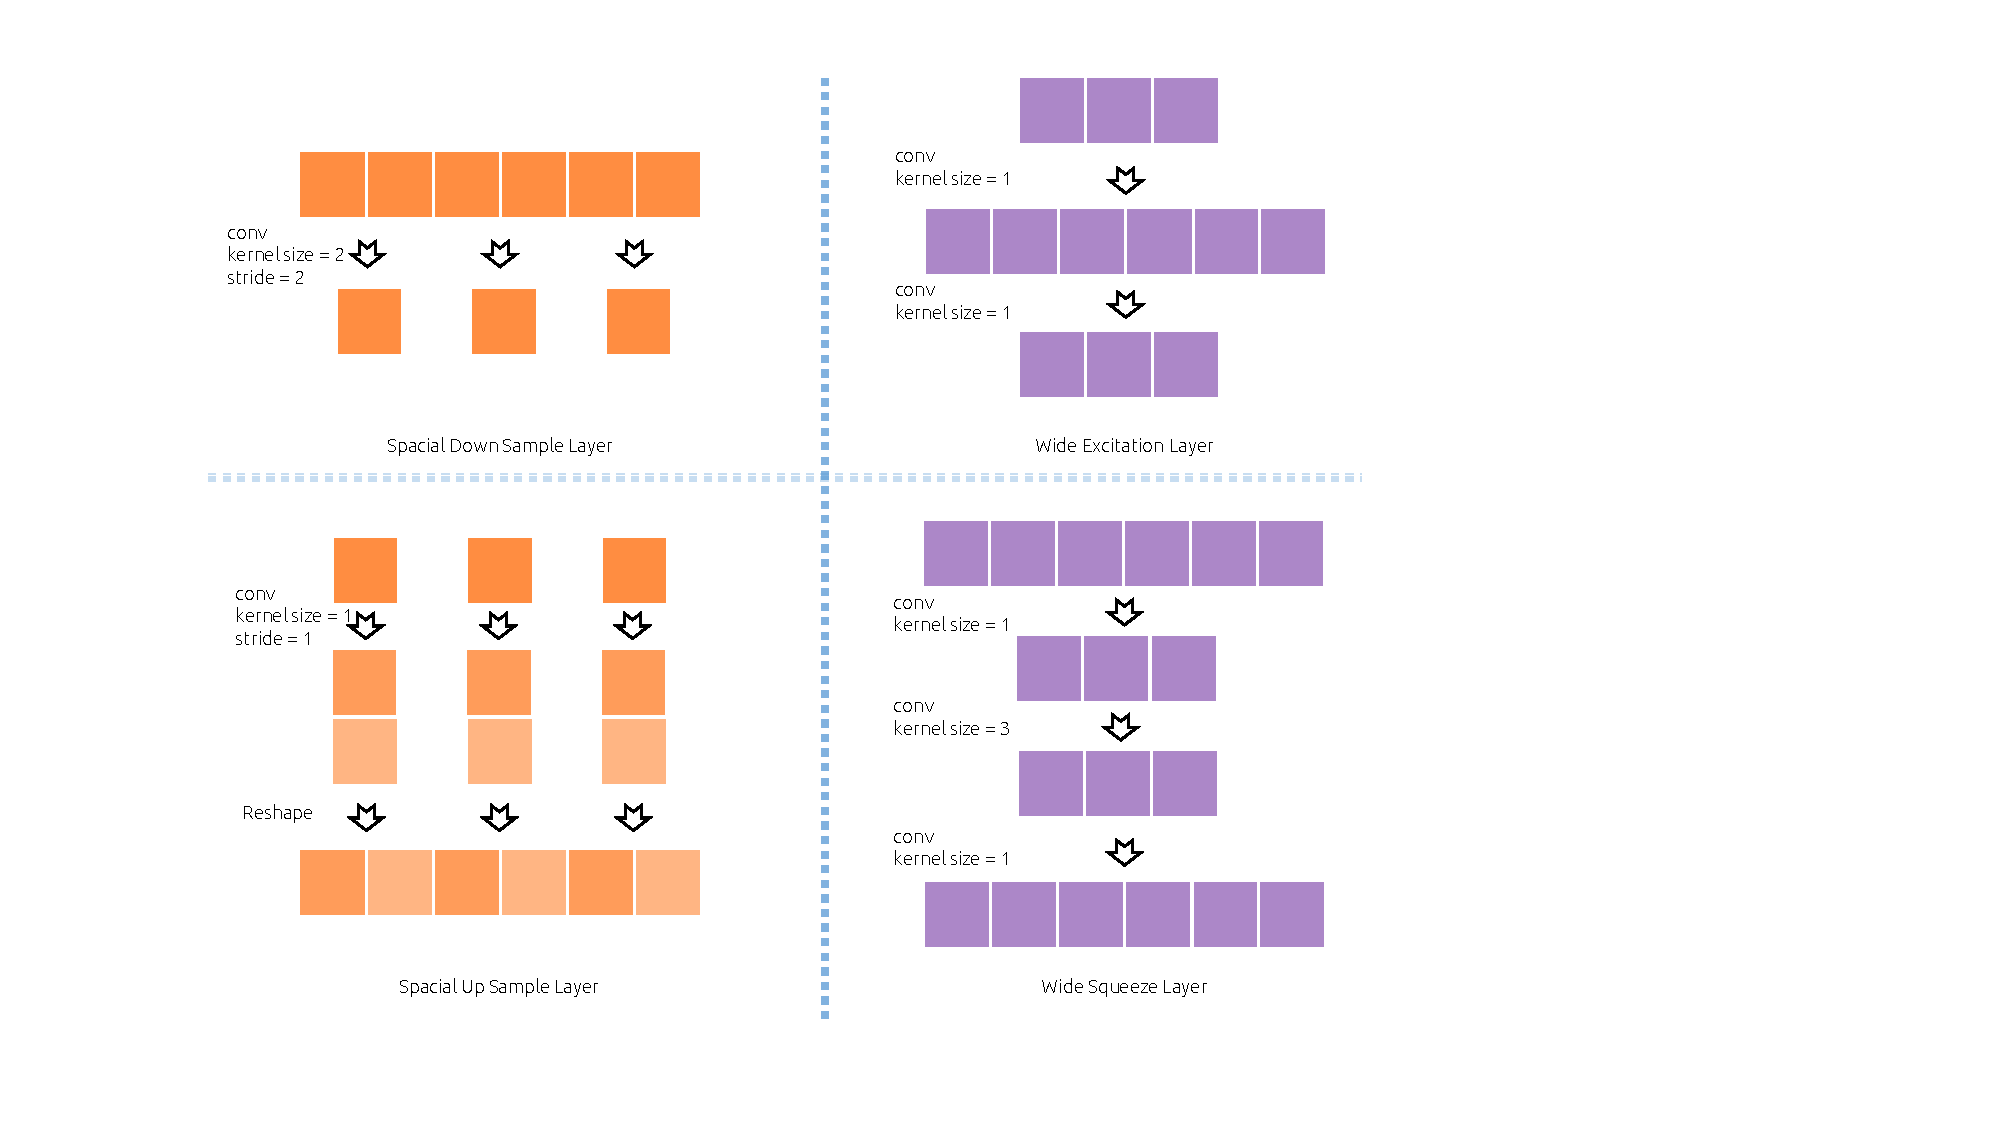
\includegraphics[width=1\linewidth]{./figs/net2.pdf}
   \caption{\textbf{The structures of up-sample, down-sample, wide expand and squeeze layers utilized in SSN and WSN. }
   Residual connection is used in both wide expand layer and wide squeeze layer across the input and output. 
   }
   \label{fig:net2}
\end{figure}


%------------------------------------------------------------------------
%-------------------------------------------------------------------------
\subsection{Margins and page numbering}


%-------------------------------------------------------------------------
\subsection{Type style and fonts}



%-------------------------------------------------------------------------
\subsection{Cross-references}

For the benefit of author(s) and readers, please use the
{\small\begin{verbatim}
  \cref{...}
\end{verbatim}}  command for cross-referencing to figures, tables, equations, or sections.
This will automatically insert the appropriate label alongside the cross-reference as in this example:
\begin{quotation}
  To see how our method outperforms previous work, please see \cref{fig:onecol} and \cref{tab:example}.
  It is also possible to refer to multiple targets as once, \eg~to \cref{fig:onecol,fig:short-a}.
  You may also return to \cref{sec:formatting} or look at \cref{eq:also-important}.
\end{quotation}
If you do not wish to abbreviate the label, for example at the beginning of the sentence, you can use the
{\small\begin{verbatim}
  \Cref{...}
\end{verbatim}}
command. Here is an example:
\begin{quotation}
  \Cref{fig:onecol} is also quite important.
\end{quotation}

%-------------------------------------------------------------------------
\subsection{References}

List and number all bibliographical references in 9-point Times, single-spaced, at the end of your paper.
When referenced in the text, enclose the citation number in square brackets, for
example~\cite{Authors14}.
Where appropriate, include page numbers and the name(s) of editors of referenced books.
When you cite multiple papers at once, please make sure that you cite them in numerical order like this \cite{Alpher02,Alpher03,Alpher05,Authors14b,Authors14}.
If you use the template as advised, this will be taken care of automatically.

\begin{table}
  \centering
  \begin{tabular}{@{}lc@{}}
    \toprule
    Method & Frobnability \\
    \midrule
    Theirs & Frumpy \\
    Yours & Frobbly \\
    Ours & Makes one's heart Frob\\
    \bottomrule
  \end{tabular}
  \caption{Results.   Ours is better.}
  \label{tab:example}
\end{table}

%-------------------------------------------------------------------------
\subsection{Illustrations, graphs, and photographs}

All graphics should be centered.
In \LaTeX, avoid using the \texttt{center} environment for this purpose, as this adds potentially unwanted whitespace.
Instead use
{\small\begin{verbatim}
  \centering
\end{verbatim}}
at the beginning of your figure.
Please ensure that any point you wish to make is resolvable in a printed copy of the paper.
Resize fonts in figures to match the font in the body text, and choose line widths that render effectively in print.
Readers (and reviewers), even of an electronic copy, may choose to print your paper in order to read it.
You cannot insist that they do otherwise, and therefore must not assume that they can zoom in to see tiny details on a graphic.

When placing figures in \LaTeX, it's almost always best to use \verb+\includegraphics+, and to specify the figure width as a multiple of the line width as in the example below
{\small\begin{verbatim}
   \usepackage{graphicx} ...
   \includegraphics[width=0.8\linewidth]
                   {myfile.pdf}
\end{verbatim}
}


%-------------------------------------------------------------------------
\subsection{Color}

Please refer to the author guidelines on the \confName\ \confYear\ web page for a discussion of the use of color in your document.

If you use color in your plots, please keep in mind that a significant subset of reviewers and readers may have a color vision deficiency; red-green blindness is the most frequent kind.
Hence avoid relying only on color as the discriminative feature in plots (such as red \vs green lines), but add a second discriminative feature to ease disambiguation.

%------------------------------------------------------------------------
\section{Final copy}

You must include your signed IEEE copyright release form when you submit your finished paper.
We MUST have this form before your paper can be published in the proceedings.

Please direct any questions to the production editor in charge of these proceedings at the IEEE Computer Society Press:
\url{https://www.computer.org/about/contact}.


%%%%%%%%% REFERENCES
{\small
\bibliographystyle{ieee_fullname}
\bibliography{egbib}
}

\end{document}
